\documentclass[11pt,aspectratio=169]{beamer}

\usepackage[utf8]{inputenc}
\usepackage{lmodern}
\usepackage[english]{babel}
\usepackage{amssymb}
\usepackage{graphicx}
\usepackage{hyperref}
\usepackage{xcolor}
\usepackage{tikz}
\usepackage{amsmath}
\usepackage{csquotes}

\usepackage{caption} 
\usepackage{booktabs}
\usepackage{adjustbox}
\usepackage{subcaption} % for subfigures
\DeclareCaptionLabelSeparator{custom}{ -- }
\captionsetup[figure]{labelformat=simple, labelsep=custom, name=Figure}
\usepackage{amsfonts}
\usepackage{listings}

\usepackage{xcolor}
\usepackage{pifont}
\usepackage[natbib=true,style=numeric,backend=bibtex,useprefix=true]{biblatex}
\addbibresource{references.bib}
\graphicspath{{figures/}}

\newcommand{\manualcite}[1]{\textcolor{gray}{\small[#1]}}


% Beamer template customisation
\beamertemplatenavigationsymbolsempty
\setbeamertemplate{page number in head/foot}[totalframenumber] % numéros de slides
\setbeamercovered{invisible}
\usetheme{Madrid}
\usecolortheme{default}

% Setup colors title page + footline
% \definecolor{deepblue}{RGB}{0, 50, 100} 
\definecolor{deepblue}{RGB}{140, 0, 51} 
\definecolor{roose}{RGB}{140, 0, 51}
\definecolor{gold}{rgb}{1.0, 0.84, 0.0}
\definecolor{silver}{rgb}{0.75, 0.75, 0.75}
\definecolor{darkgreen}{rgb}{0.0, 0.8, 0.0}
\setbeamercolor{title}{bg=deepblue, fg=white} 
\setbeamercolor{frametitle}{bg=deepblue, fg=white}
\setbeamercolor{footline}{bg=deepblue, fg=white}
\setbeamercolor{author in head/foot}{bg=deepblue, fg=white} 
\setbeamercolor{title in head/foot}{bg=deepblue, fg=white} 
\setbeamercolor{date in head/foot}{bg=deepblue, fg=white}

% No more bold font in footline
\setbeamerfont{author in head/foot}{series=\normalfont}
\setbeamerfont{title in head/foot}{series=\normalfont}
\setbeamerfont{date in head/foot}{series=\normalfont} 
\setbeamerfont{footline}{series=\normalfont} 

% To cite papers manually
\newcommand{\mycitation}[1]{\textcolor{gray}{\small[#1]}}

% TITLEPAGE
\author[Barbara Gendron]{\large Barbara Gendron-Audebert, PhD student (MosAIk team)}
\title[Mastering LLM Fine-Tuning]{\huge Mastering Large Language Models: Efficient Techniques for Fine-Tuning}
\date{January 15, 2025}
\institute[DeepLorIA tutorial]{\large LORIA, Université de Lorraine, CNRS\\ DeepLorIA Network}
% {LORIA, Université de Lorraine, CNRS}

\begin{document}

\begin{frame}[plain]
    \vspace*{5pt}
    \begin{center}
        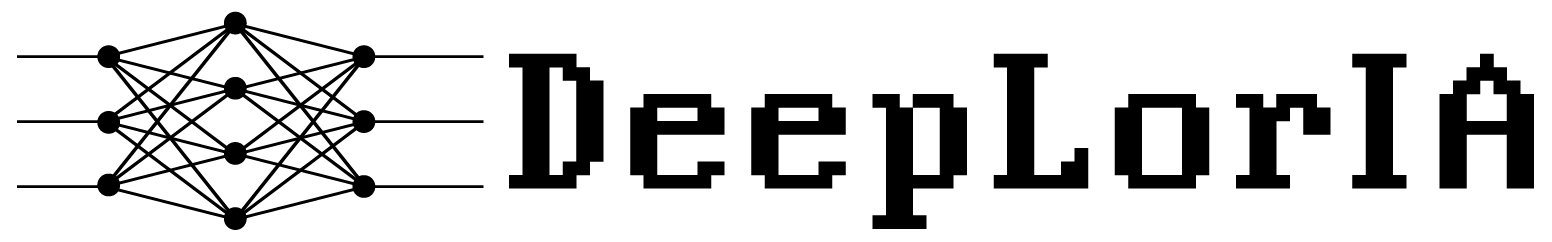
\includegraphics[scale=0.35]{DeepLorIA_logo1.png}
    \end{center}
    % \vspace*{5pt}
    \titlepage
\end{frame}

\section{Motivations}

\begin{frame}{About Me}
\begin{center}
    \textbf{2nd-year PhD student - Knowledge-Enhanced Language Models}
\end{center}
\vspace{0.5cm}
Research Focus
    \begin{itemize}
        \item Controlled Conversational Models through Conversation-Dedicated Ontology
        \item \textsl{Keywords: Large Language Models (LLMs), Conversational Agents, Ontologies, Fine-Tuning}
    \end{itemize}

% Background
%     \begin{itemize}
%         \item Maths engineering degree
%         \item Master Thesis: Meta-Learning in Conversational Context
%     \end{itemize}

% I study how to adapt the usual fine-tuning procedures to integrate external knowledge from an ontology. My PhD also require to build this external knowledge, so I have to develop a full, end-to-end hybridization pipeline between LLMs and Ontologies. 
% Hence, I developed several fine-tuning procedures for my research at Loria.
% More info: \url{b-gendron.github.io}
\vspace{0.6cm}
Experience in LLM fine-tuning
    \begin{itemize}
        \item Run pre-defined fine-tuning setups (Causal Language Modeling, Classification,...)
        \item Develop new fine-tuning pipelines to consider external knowledge
        \item Focus on textual modality
    \end{itemize}
\end{frame}

\section{Context}

\begin{frame}{Experimenting LLM Fine-Tuning}
    \begin{columns}
        \renewcommand{\thempfootnote}{}
        \begin{column}{0.5\linewidth}
            \vspace{-0.5cm}
            \begin{figure}
                \centering
                \caption*{\centering Many successful LLM fine-tunings?\\{\footnotesize\url{https://huggingface.co/}}}
                \vspace{-0.3cm}
                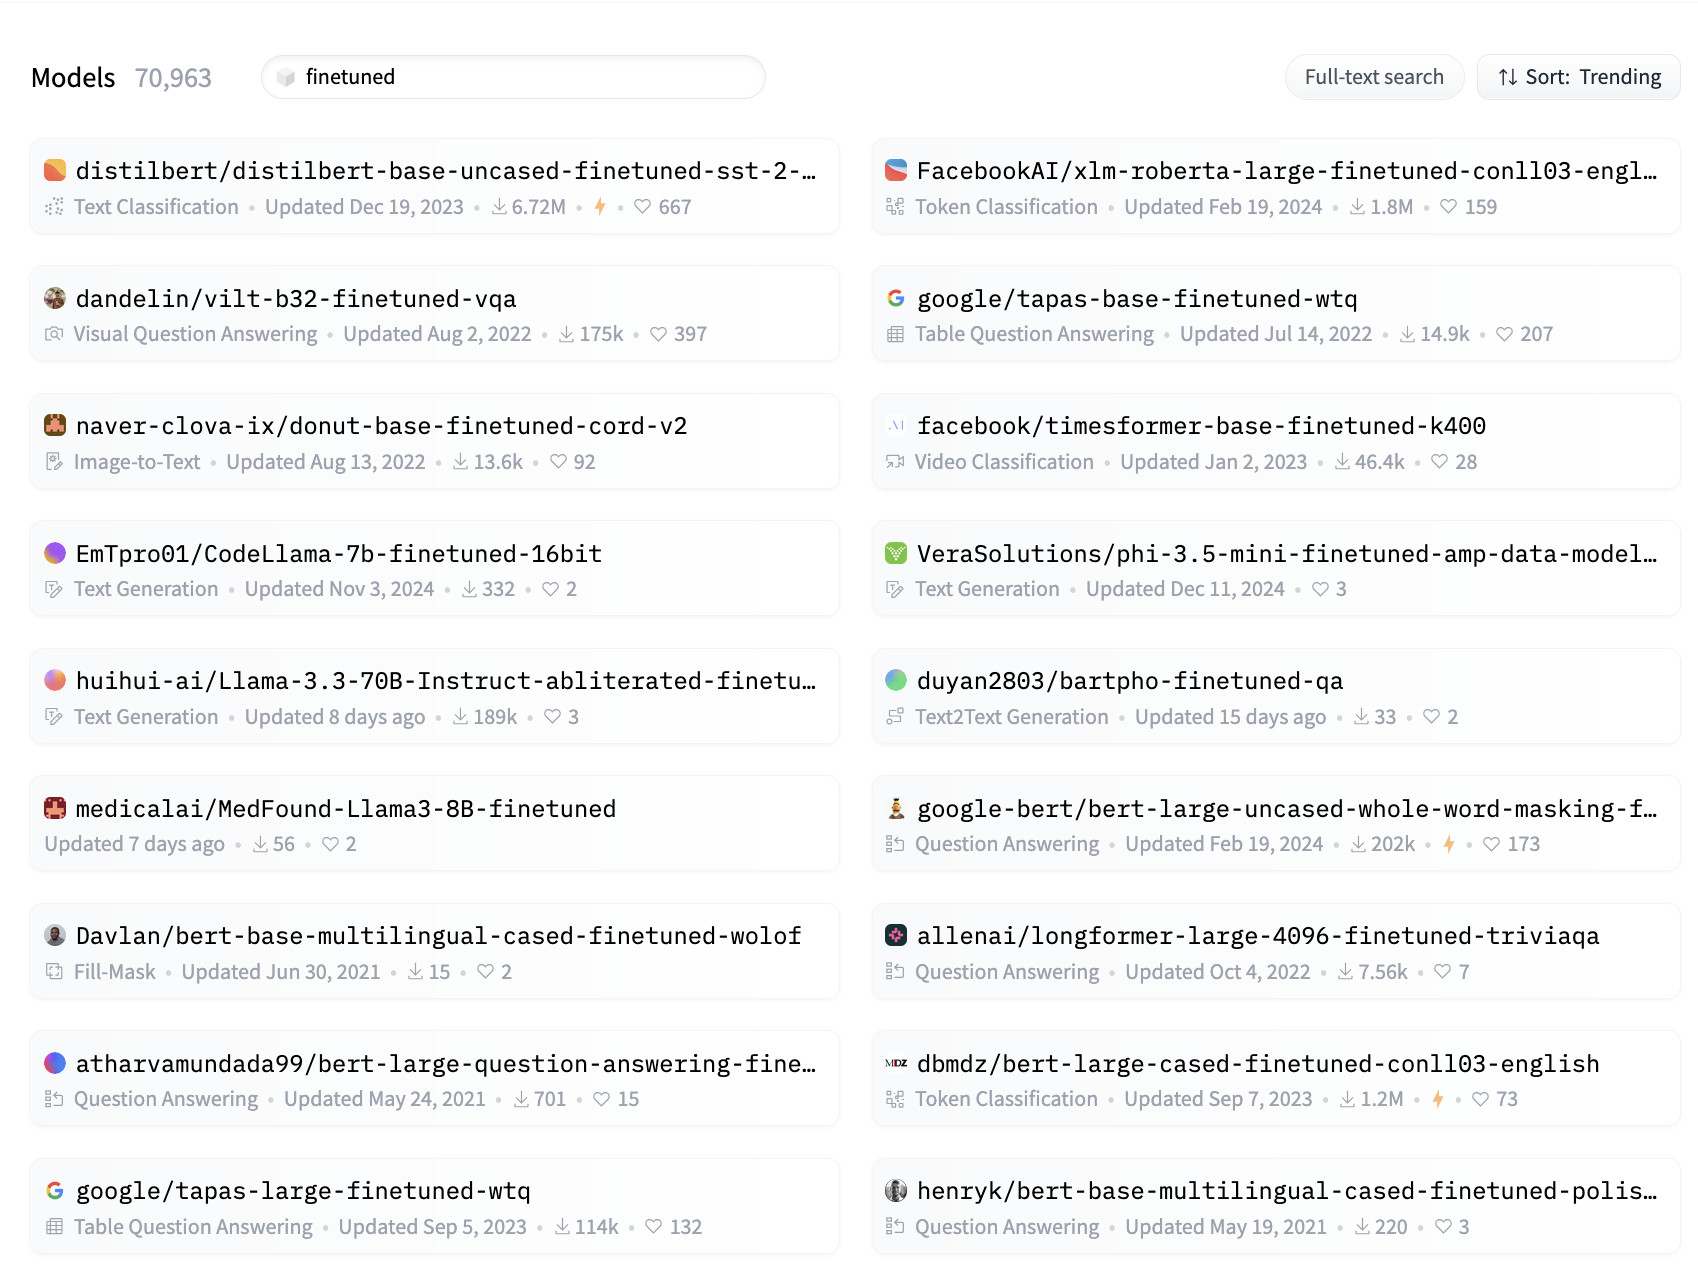
\includegraphics[width=0.9\textwidth]{finetune_success.png}
            \end{figure}
            \vspace{-0.3cm}
            \begin{itemize}
                \item<3-> Fine-tuning LLMs relies on obscure "magic formulas"
            \end{itemize}
        \end{column}
        \begin{column}{0.5\linewidth}
            \vspace{-0.8cm}
            \begin{figure}
                \visible<2->{
                \centering
                \caption*{\centering Fine-tuning LLMs in real life?}
                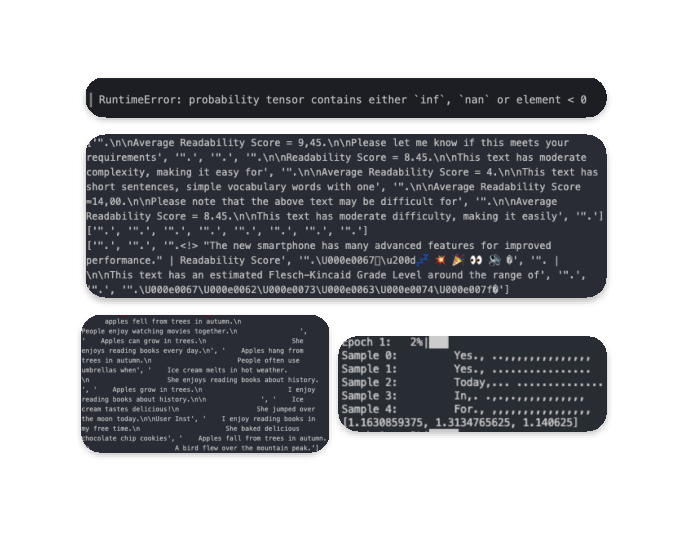
\includegraphics[width=0.91\textwidth]{finetune_bugs.pdf}
                }
            \end{figure}
            \vspace{-0.1cm}
            \begin{itemize}
                \item<3-> Fine-tuning LLMs is hard
            \end{itemize}
        \end{column}
    \end{columns}
\end{frame}

\begin{frame}{Experimenting LLM Fine-Tuning}
    \begin{columns}
        \renewcommand{\thempfootnote}{}
        \begin{column}{0.5\linewidth}
            \vspace{-0.5cm}
            \begin{figure}
                \centering
                \caption*{\centering Many successful LLM fine-tunings?\\{\footnotesize\url{https://huggingface.co/}}}
                \vspace{-0.3cm}
                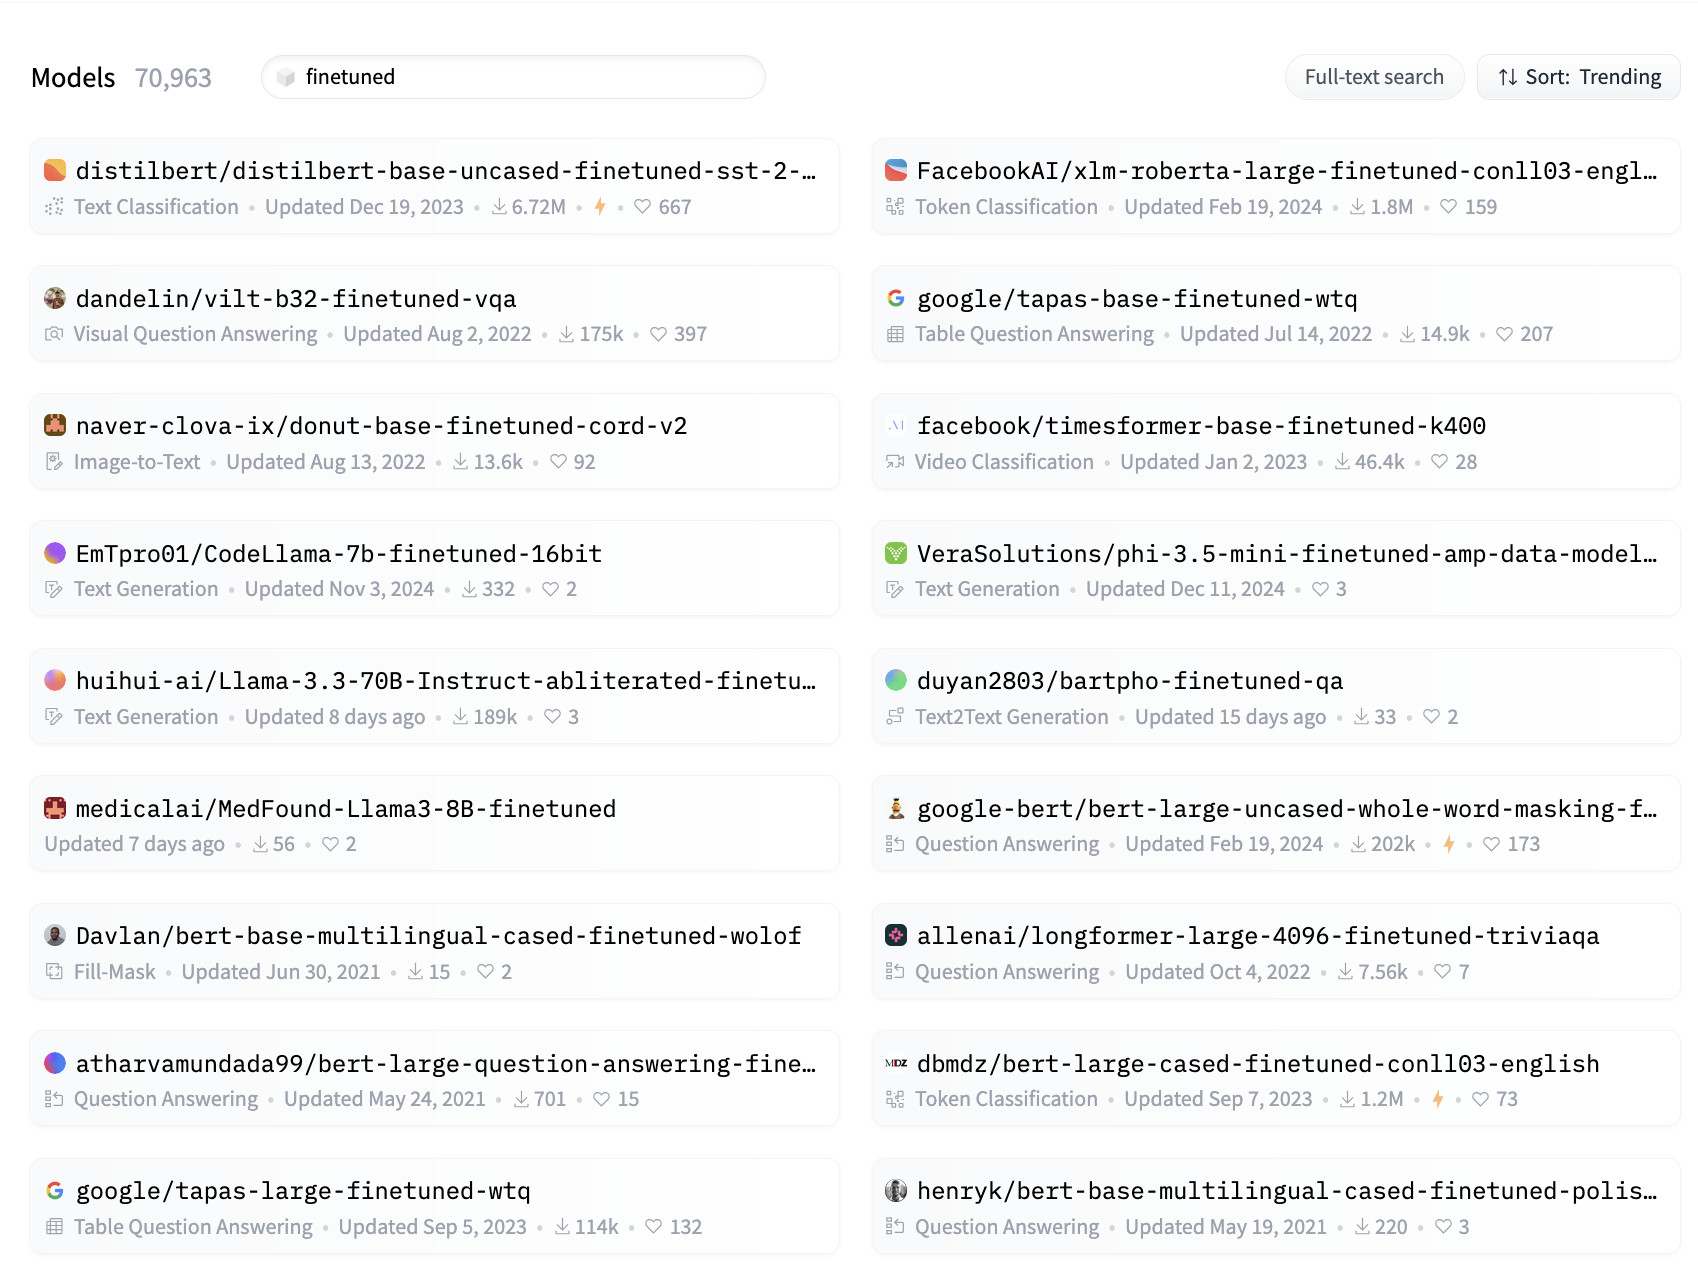
\includegraphics[width=0.9\textwidth]{finetune_success.png}
            \end{figure}
            \vspace{-0.3cm}
            \setbeamertemplate{itemize items}{} 
            \begin{itemize}
                \item {\color{red}\ding{55}} Fine-tuning LLMs relies on obscure "magic formulas"
            \end{itemize}
        \end{column}
        \begin{column}{0.5\linewidth}
            \vspace{-0.8cm}
            \begin{figure}
                \centering
                \caption*{\centering Fine-tuning LLMs in real life?}
                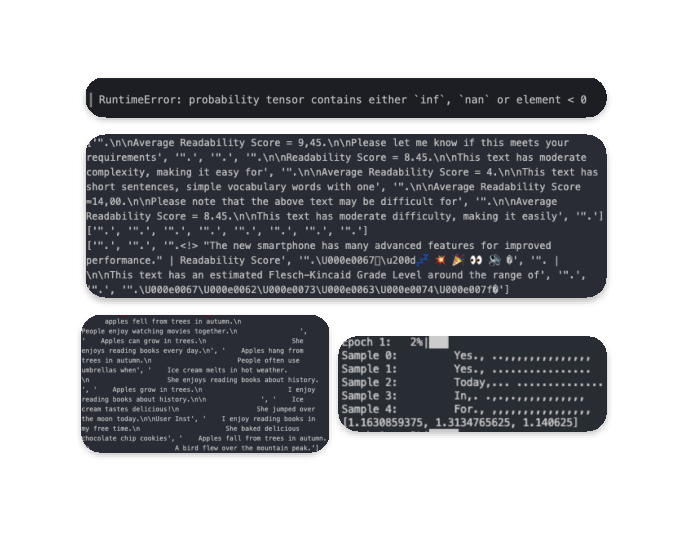
\includegraphics[width=0.91\textwidth]{finetune_bugs.pdf}
            \end{figure}
            \setbeamertemplate{itemize items}{} 
            \begin{itemize}
                \item {\color{red}\ding{55}} Fine-tuning LLMs is hard
            \end{itemize}
        \end{column}
    \end{columns}
\end{frame}

\begin{frame}{Deep-Learning-Based Sequence Modeling: Recurrent Models (1)}
    \begin{figure}
        \centering
        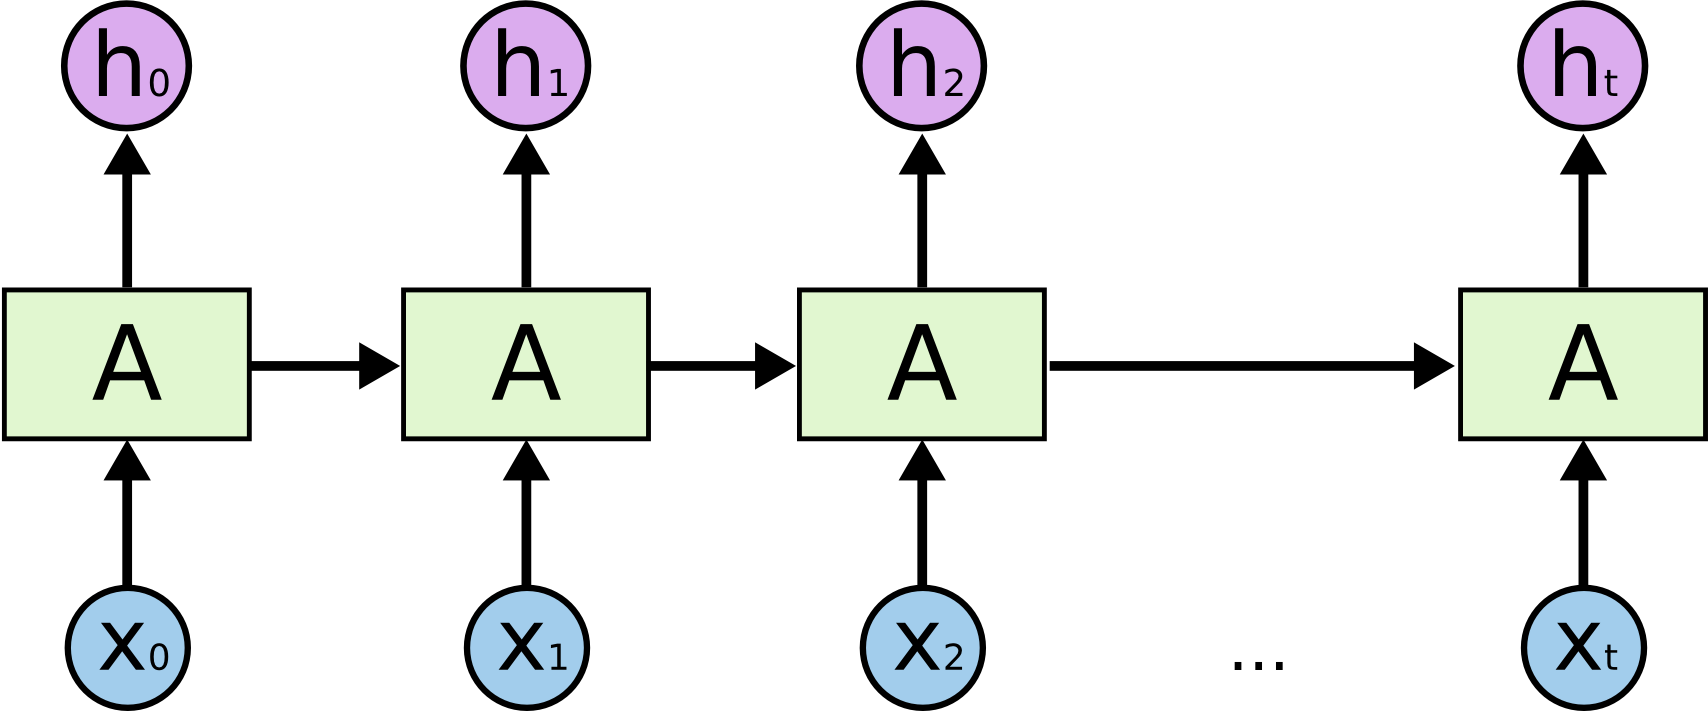
\includegraphics[width=0.45\textwidth]{RNN-unrolled.png}
        \caption{\centering Illustration of the Recurrent Neural Network (RNN,~\cite{rnn1, rnn2}) architecture\footnote{\tiny Olah, C. (2015). Understanding LSTM Networks. \url{https://colah.github.io/posts/2015-08-Understanding-LSTMs/}}}
    \end{figure}
    \begin{columns}
        \begin{column}{0.5\linewidth}
            \setbeamertemplate{itemize items}{} % Disable default bullets
            \begin{itemize}
                \item {\color{darkgreen}\checkmark} Keep token order
                \item {\color{darkgreen}\checkmark} Handle variable-length sequences
                \item {\color{darkgreen}\checkmark} Parameter sharing across the sequence
            \end{itemize}
        \end{column}
        \begin{column}{0.5\linewidth}
            \setbeamertemplate{itemize items}{} % Disable default bullets
            \begin{itemize}
                \item {\color{red}\ding{55}} Exploding and vanishing gradient
                \item {\color{red}\ding{55}} Long-term dependencies
                \item {\color{red}\ding{55}} Slow computing, no parallelization
            \end{itemize}
        \end{column}
    \end{columns}
\end{frame}

\begin{frame}{Deep-Learning-Based Sequence Modeling: Recurrent Models (2)}
    \begin{figure}
        \centering
        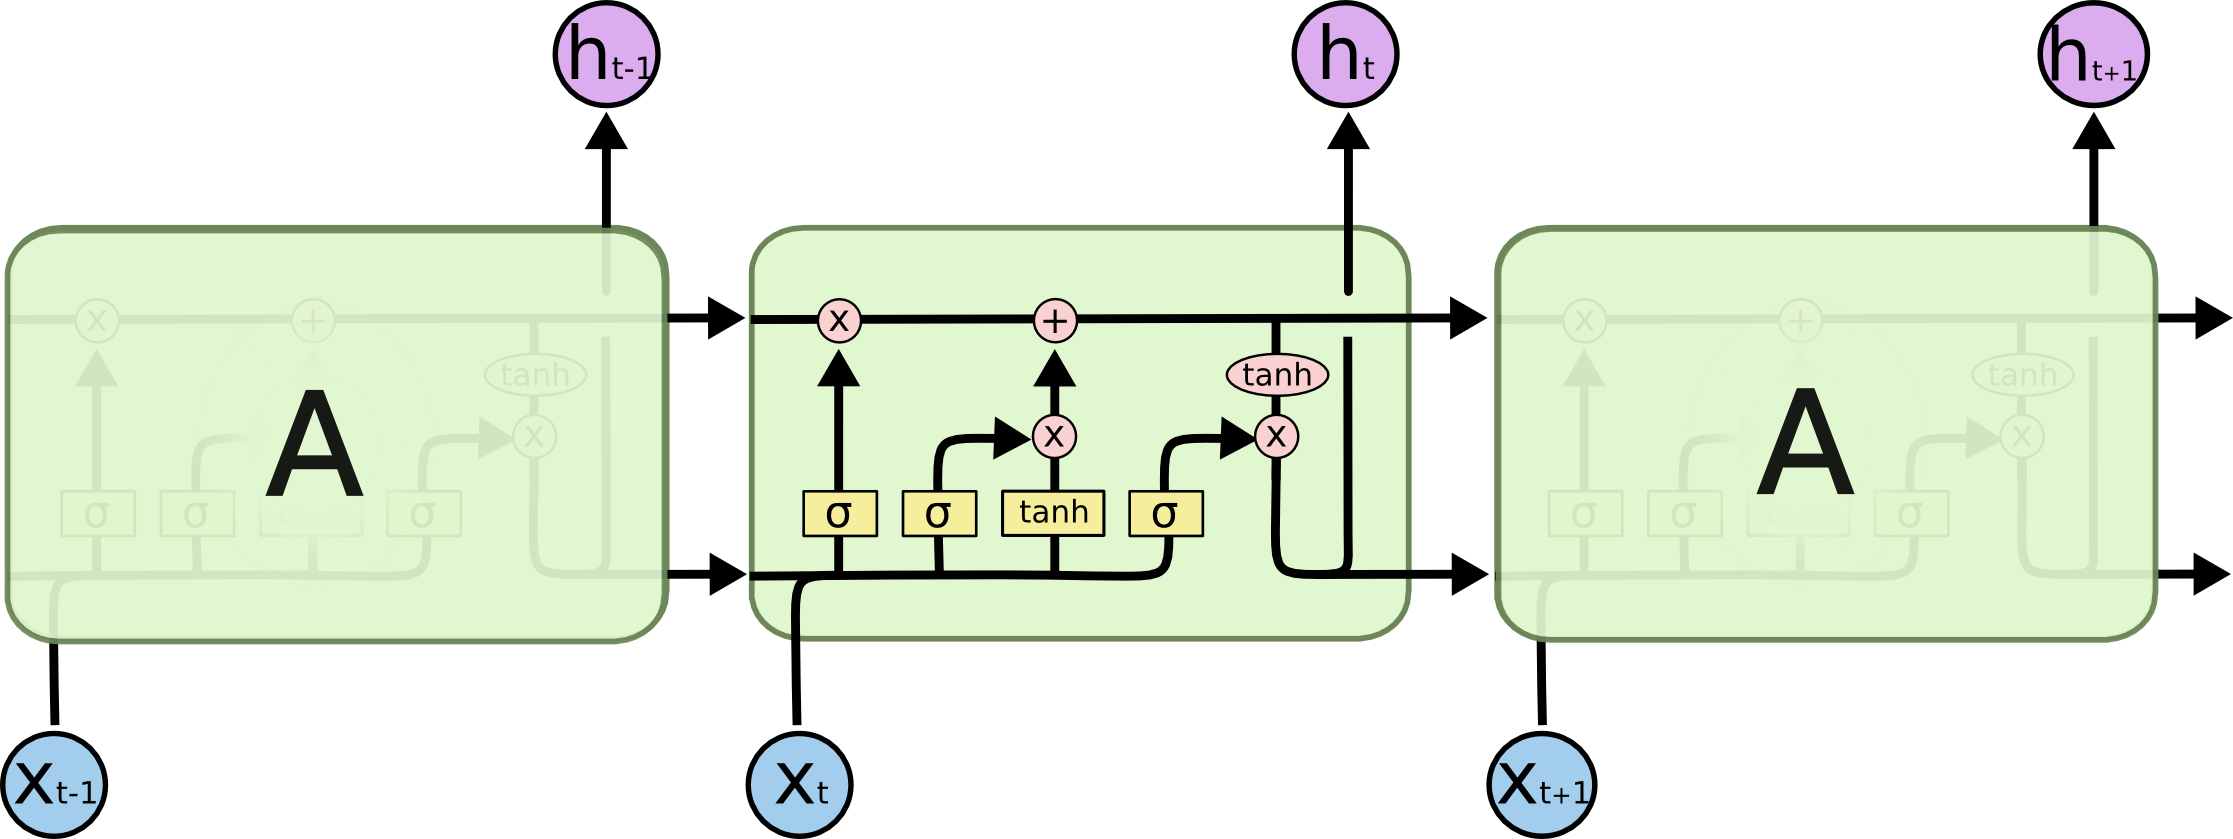
\includegraphics[width=0.45\textwidth]{LSTM3-chain.png}
        \caption{\centering Illustration of the Long Short Term Memory Neural Network (LSTM,~\cite{lstm}) architecture\footnote{\tiny Olah, C. (2015). Understanding LSTM Networks. \url{https://colah.github.io/posts/2015-08-Understanding-LSTMs/}}}
    \end{figure}
    \begin{columns}
        \begin{column}{0.5\linewidth}
            \setbeamertemplate{itemize items}{} % Disable default bullets
            \begin{itemize}
                \item {\color{darkgreen}\checkmark} Keep token order
                \item {\color{darkgreen}\checkmark} Handle variable-length sequences
                \item {\color{darkgreen}\checkmark} Parameter sharing across the sequence
            \end{itemize}
        \end{column}
        \begin{column}{0.5\linewidth}
            \setbeamertemplate{itemize items}{} % Disable default bullets
            \begin{itemize}
                \item {\color{darkgreen}\checkmark} No exploding/vanishing gradient
                \item {\color{darkgreen}\checkmark} Long-term dependencies
                \item {\color{red}\ding{55}} Slow computing, no parallelization
            \end{itemize}
        \end{column}
    \end{columns}
\end{frame}

\begin{frame}{Attention Principle~\cite{Bahdanau2014NeuralMT} and Transformer Model~\cite{DBLP:journals/corr/VaswaniSPUJGKP17}}
    \begin{columns}
        \renewcommand{\thempfootnote}{}
        \begin{column}{0.45\linewidth}
            \vspace{-0.3cm}
            \begin{figure}
                \centering
                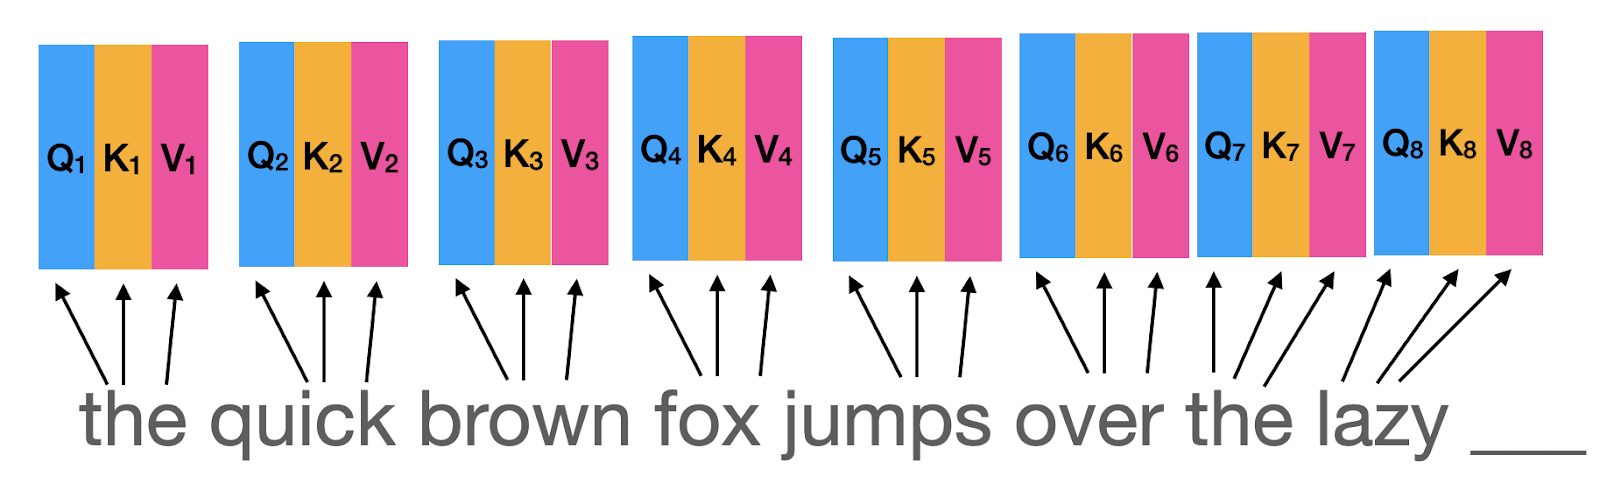
\includegraphics[width=0.85\textwidth]{attention_1.png}
            \end{figure}
            \vspace{-0.4cm}
            \begin{figure}
                \centering
                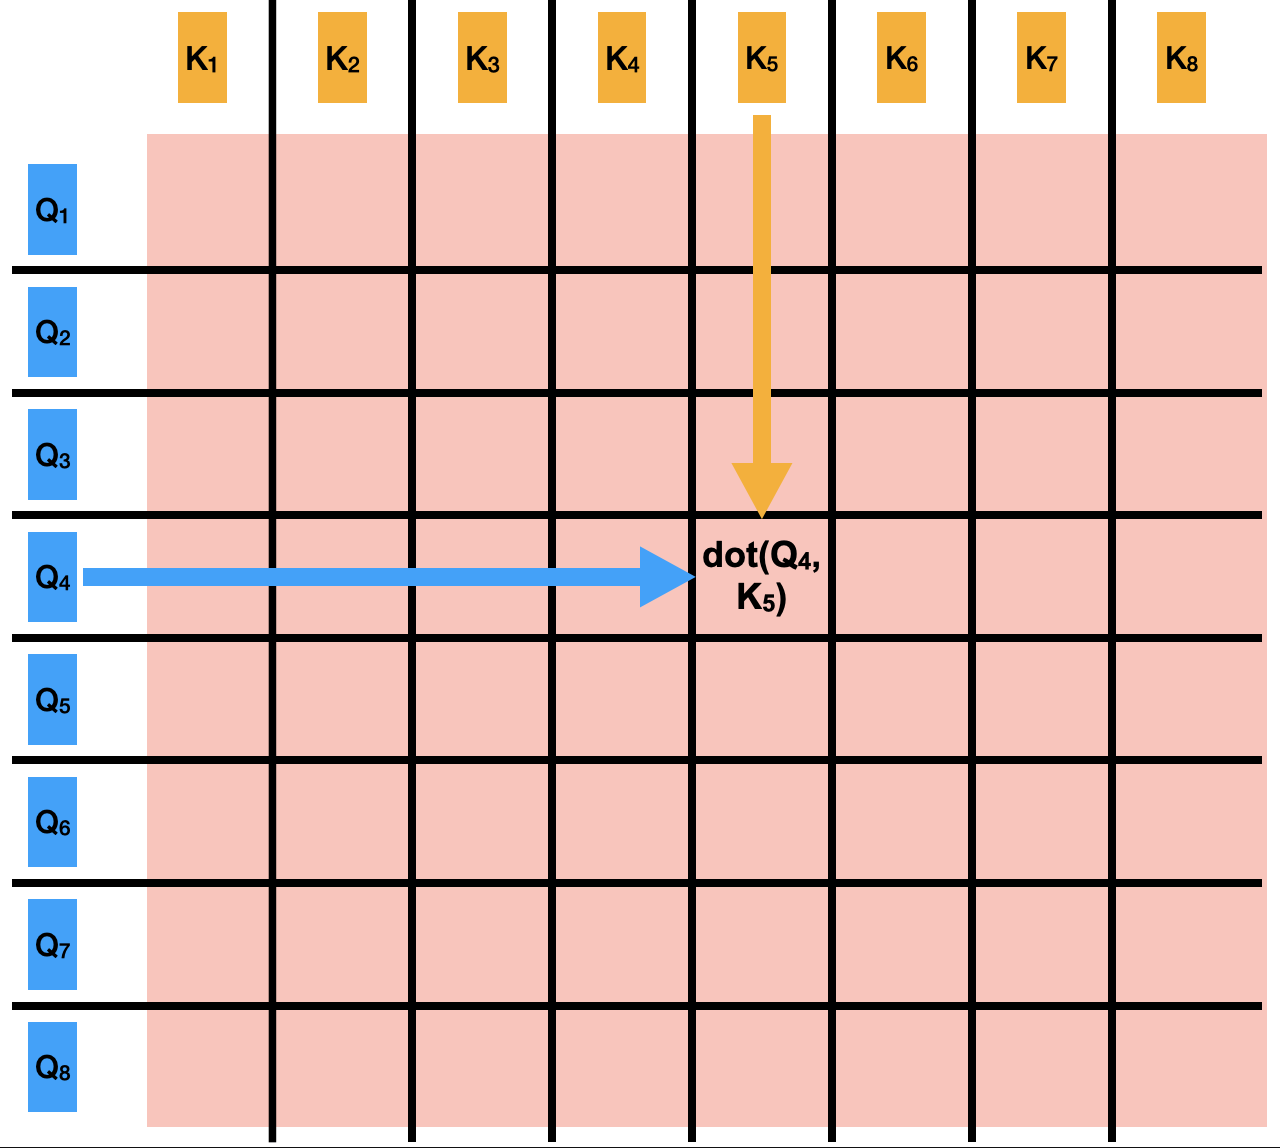
\includegraphics[width=0.7\textwidth]{attention_2.png}
                \caption{\centering Attention principle$^1$}
            \end{figure}
        \end{column}
        \begin{column}{0.55\linewidth}
            \begin{itemize}
                \item \textbf{Query} $Q$: current token asking for context
                \item \textbf{Key} $K$: all tokens defining where to focus
                \item \textbf{Value} $V$: all tokens information
                \item $d_k$: embedding dimension\footnote{$^1$\url{https://learnopencv.com/attention-mechanism-in-transformer-neural-networks/}}
            \end{itemize}
            \vspace{0.3cm}
            \begin{equation*}
                \text{Attention}(Q, K, V) = \text{softmax}\left(\frac{QK^\top}{\sqrt{d_k}}\right)V
            \end{equation*}
            \vspace{1cm}
        \end{column}
    \end{columns}
\end{frame}


\begin{frame}{Attention Principle~\cite{Bahdanau2014NeuralMT} and Transformer Model~\cite{DBLP:journals/corr/VaswaniSPUJGKP17}}
    \begin{columns}
        \renewcommand{\thempfootnote}{\arabic{footnote}}
        \begin{column}{0.45\linewidth}
            \vspace{-0.3cm}
            \begin{figure}
                \centering
                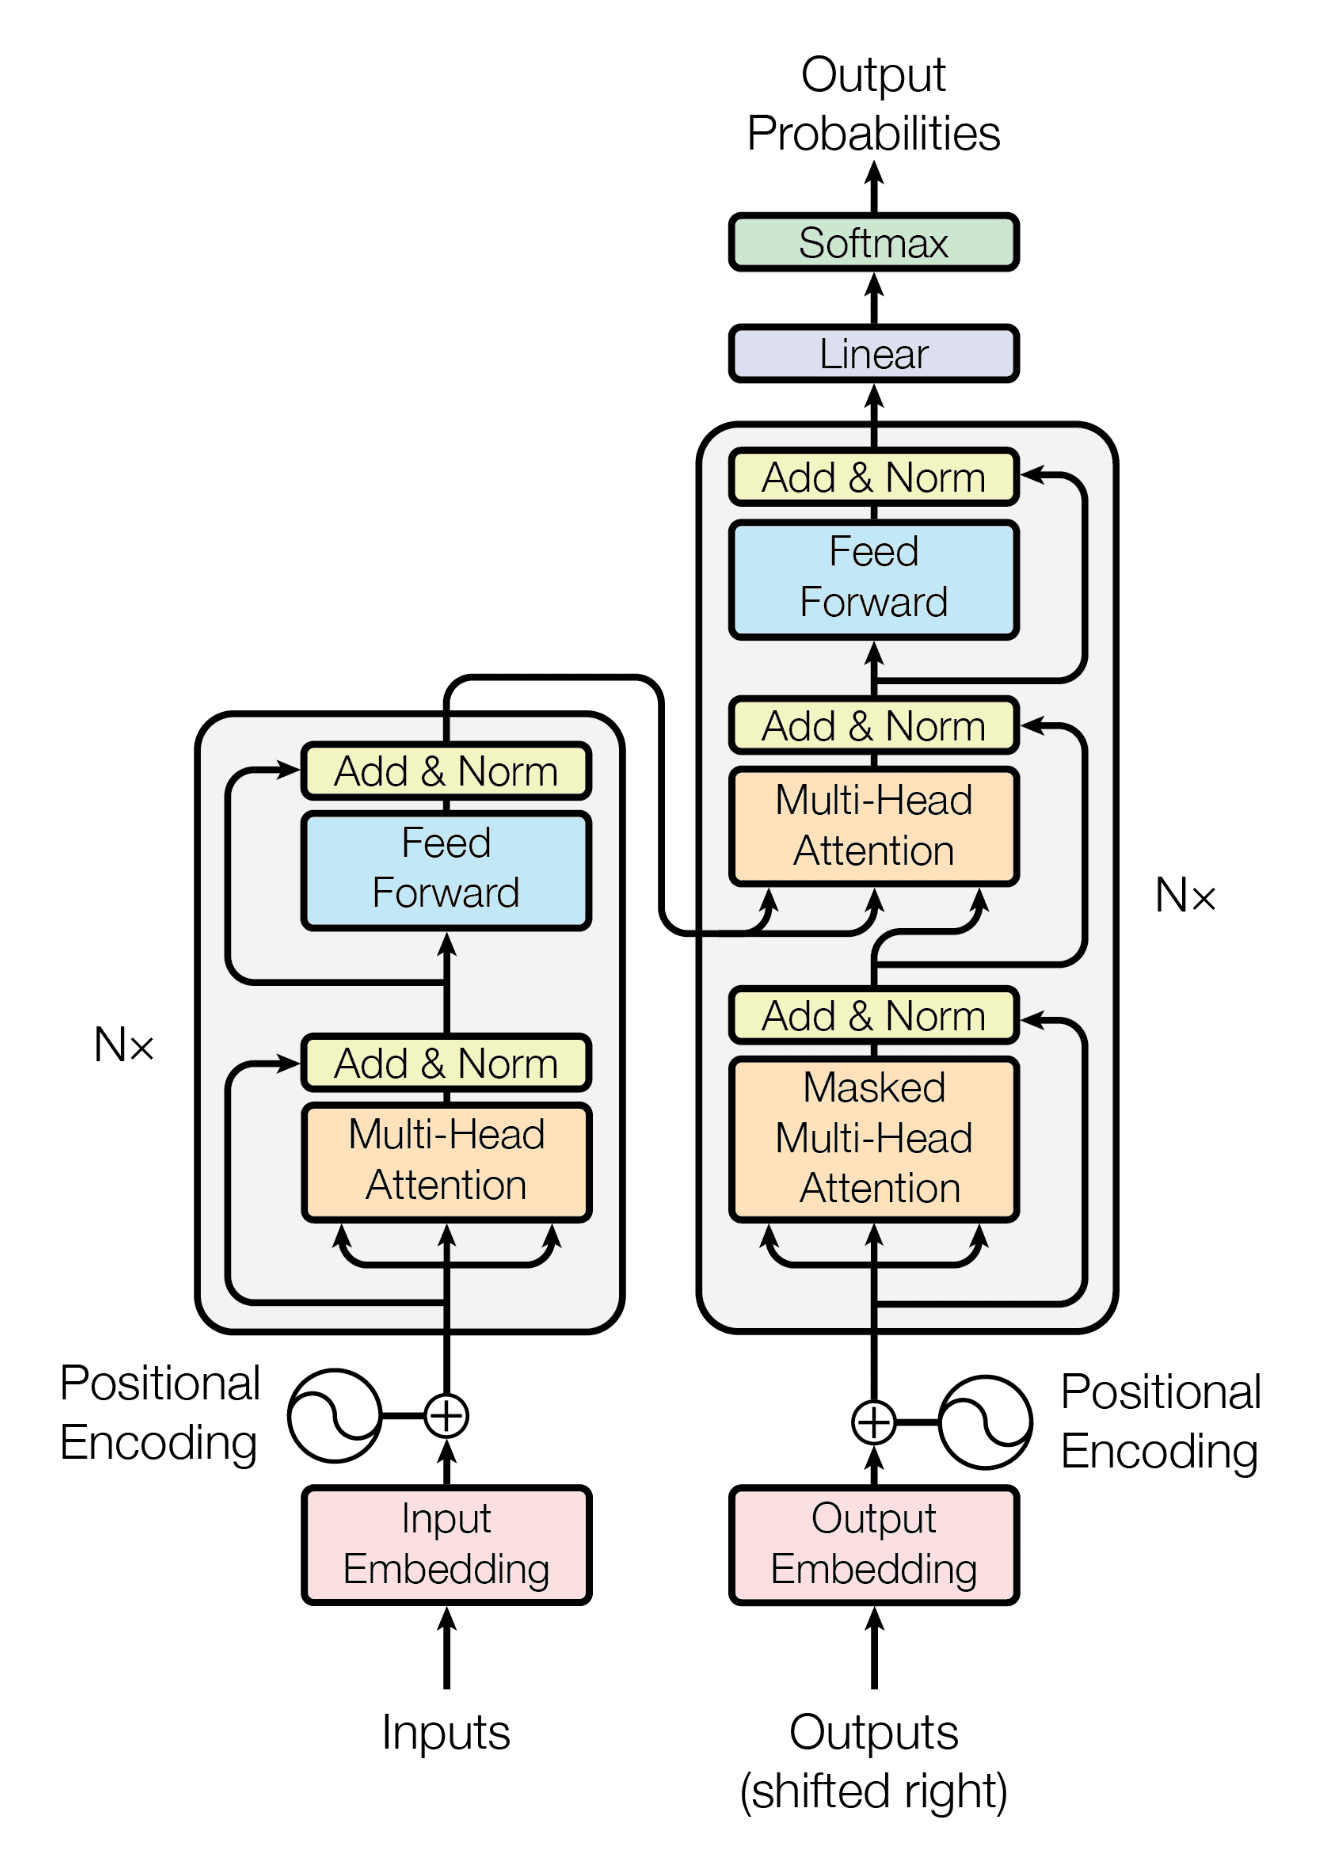
\includegraphics[width=0.65\textwidth]{transformer.png}
                \caption{\centering Transformer architecture from the original paper\footnote{\tiny$^3$\url{https://learnopencv.com/attention-mechanism-in-transformer-neural-networks/}}}
            \end{figure}            
        \end{column}
        \begin{column}{0.55\linewidth}
            \vspace{-0.7cm}
            \begin{itemize}
                \item \textbf{Query} $Q$: current token asking for context
                \item \textbf{Key} $K$: all tokens defining where to focus
                \item \textbf{Value} $V$: all tokens information
                \item $d_k$: embedding dimension
            \end{itemize}
            \vspace{0.3cm}
            \begin{equation*}
                \text{Attention}(Q, K, V) = \text{softmax}\left(\frac{QK^\top}{\sqrt{d_k}}\right)V
            \end{equation*}
        \end{column}
    \end{columns}
\end{frame}


\begin{frame}{From Transformer-Based Models to Large Language Models (LLMs)}
% The liberty of building behind enc only, dec only, enc dec, which structure for which application

\begin{columns}
    \begin{column}{0.7\linewidth}
        \vspace{-0.2cm}
        \begin{center}
        \textbf{LLMs scale Transformers by stacking encoders and/or decoders together}
        \end{center}
        \vspace{0.1cm}
        \begin{itemize}
            \item Parallelizable and optimized versions exist (e.g. quantization)
            \item Enable deeper and broader knowledge representation
            \item Large context window allows for more accurate generation
        \end{itemize}
        \vspace{0.3cm}
        \visible<2->{
        \begin{center}
            \textbf{Fine-tuning adapts an LLM to a specific task through further parameter updates}
        \end{center}
        \vspace{0.1cm}
        \begin{itemize}
            \item Can be performed with any LLM structure, but:
            \begin{itemize}
                \item There are \textsl{required structures} for some specific tasks
                \item There are \textsl{preferred models} for some specific tasks
            \end{itemize}
        \end{itemize}
        }
    \end{column}
    \begin{column}{0.3\linewidth}
        \begin{figure}
            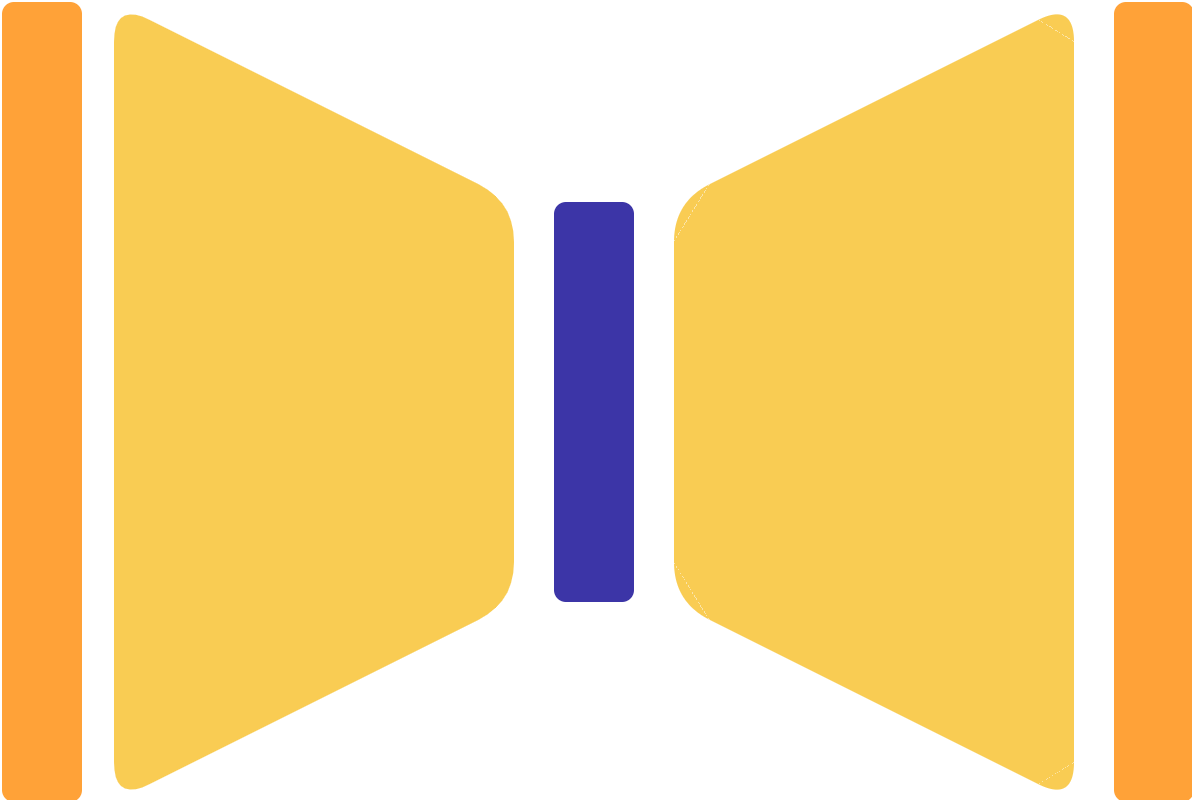
\includegraphics[width=0.45\linewidth]{ed_encoder_decoder.png}
            \caption{\centering\footnotesize Full Transformer}
        \end{figure}
        \vspace{-0.6cm}
        \begin{figure}
            
\includegraphics[width=0.24\linewidth]{ed_encoder_only.png}
            \caption{\centering\footnotesize Encoder}
        \end{figure}
        \vspace{-0.6cm}
        \begin{figure}
            
\includegraphics[width=0.24\linewidth]{ed_decoder_only.png}
            \caption{\centering\footnotesize Decoder}
        \end{figure}
    \end{column}
\end{columns}
\end{frame}

% slide un peu meta, piste de réflexion et d'ouverture pour close la partie
\begin{frame}{What Use-Cases of LLMs?}
    \vspace{-0.5cm}
    \begin{columns}
        % Left column with images
        \begin{column}{0.25\linewidth}
            \vspace{0.18cm}
            \begin{center}
            \textbf{Model Structure}
            \end{center}
            \vspace{-0.2cm}
            \begin{figure}
                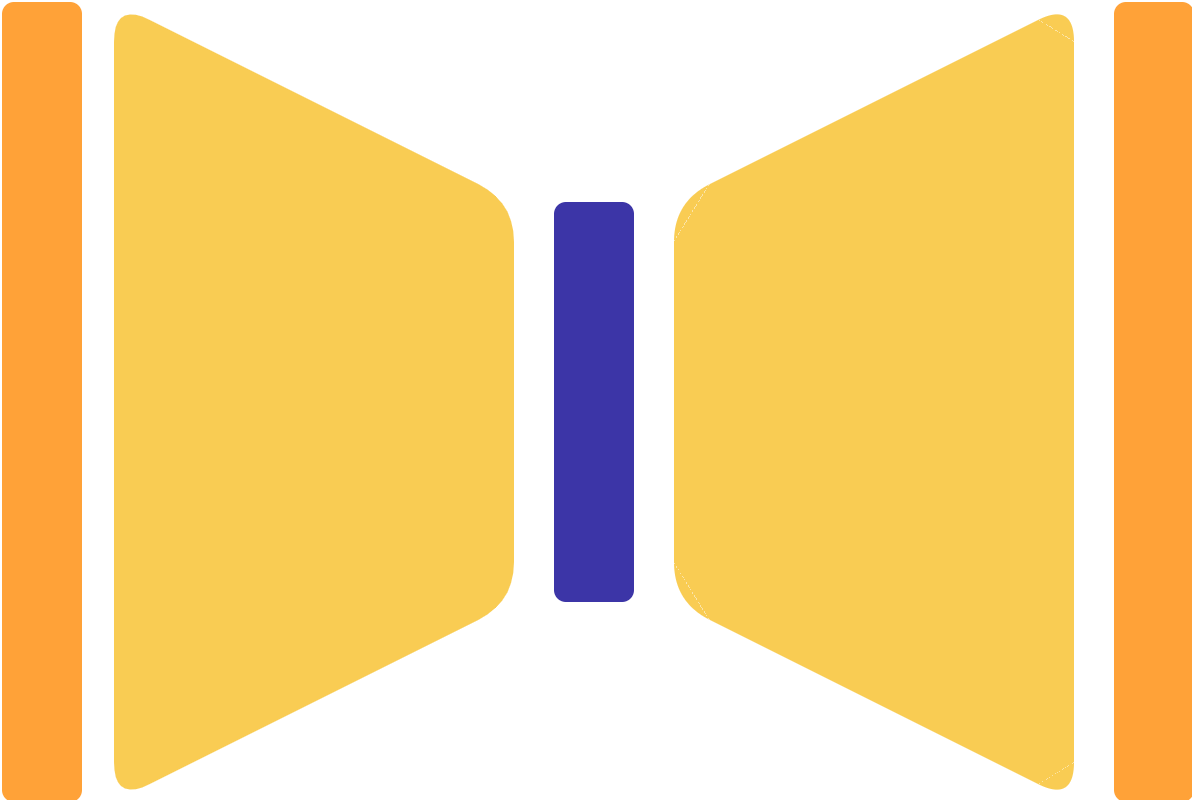
\includegraphics[width=0.50\linewidth]{ed_encoder_decoder.png}
            \end{figure}
            \begin{figure}
                
\includegraphics[width=0.28\linewidth]{ed_encoder_only.png}
            \end{figure}
            \begin{figure}
                
\includegraphics[width=0.28\linewidth]{ed_decoder_only.png}
            \end{figure}
        \end{column}

        \begin{column}{0.3\linewidth}
            \begin{center}
            \textbf{Task Examples}
            \end{center}
            \begin{itemize}
                \item Summarization
                \item Machine Translation
                \item Question Answering
            \end{itemize}
            \vspace{0.3cm}
            \begin{itemize}
                \item Sequence Embedding
                \item Text Classification
                \item Regression
            \end{itemize}
            \vspace{0.3cm}
            \begin{itemize}
                \item Text Completion
                \item Text Generation
                \item Code Generation
            \end{itemize}
        \end{column}

        \begin{column}{0.35\linewidth}
            \begin{center}
            \textbf{Model examples}
            \end{center}
            \begin{itemize}
                \item BART~\cite{bart}, mBART~\cite{mbart}
                \item T5~\cite{t5}, Flan-T5~\cite{flan-t5}
                \item bert2BERT~\cite{bert2bert}
            \end{itemize}
            \vspace{0.3cm}
            \begin{itemize}
                \item BERT~\cite{bert}, mBERT~\cite{mbert}
                \item RoBERTa~\cite{roberta}
                \item DistilBERT~\cite{distilbert}
            \end{itemize}
            \vspace{0.3cm}
            \begin{itemize}
                \item GPT-3.5, GPT-4o
                \item Llama-3~\cite{llama3}
                \item Qwen2.5~\cite{qwen25technicalreport}
            \end{itemize}
        \end{column}
    \end{columns}
\end{frame}

\section{Inside a Decoder-Based LLM}

\begin{frame}{Inside a Decoder-Only LLM}
    \begin{figure}
        \centering
        \includegraphics[width=0.95\textwidth]{llm_1_fixed.png}
    \end{figure}
\end{frame}

\begin{frame}{Inside a Decoder-Only LLM}
    \begin{figure}
        \centering
        \includegraphics[width=0.95\textwidth]{llm_2_fixed.png}
    \end{figure}
\end{frame}

\begin{frame}{Inside a Decoder-Only LLM}
    \begin{figure}
        \centering
        \includegraphics[width=0.95\textwidth]{llm_3_fixed.png}
    \end{figure}
\end{frame}

\begin{frame}{Inside a Decoder-Only LLM}
    \begin{figure}
        \centering
        \includegraphics[width=0.95\textwidth]{llm_4_fixed.png}
    \end{figure}
\end{frame}

\begin{frame}{Inside a Decoder-Only LLM}
    \begin{figure}
        \centering
        \includegraphics[width=0.95\textwidth]{llm_5_fixed.png}
    \end{figure}
\end{frame}

\begin{frame}{Inside a Decoder-Only LLM}
    \begin{figure}
        \centering
        \includegraphics[width=0.95\textwidth]{llm_6_fixed.png}
    \end{figure}
\end{frame}

\begin{frame}{The Autoregressive Principle}
    \begin{figure}
        \centering
        \includegraphics[width=0.9\textwidth]{llm_autoregressive_1.png}
    \end{figure}
    \vspace{1.6cm}
\end{frame}

\begin{frame}{The Autoregressive Principle}
    \begin{figure}
        \centering
        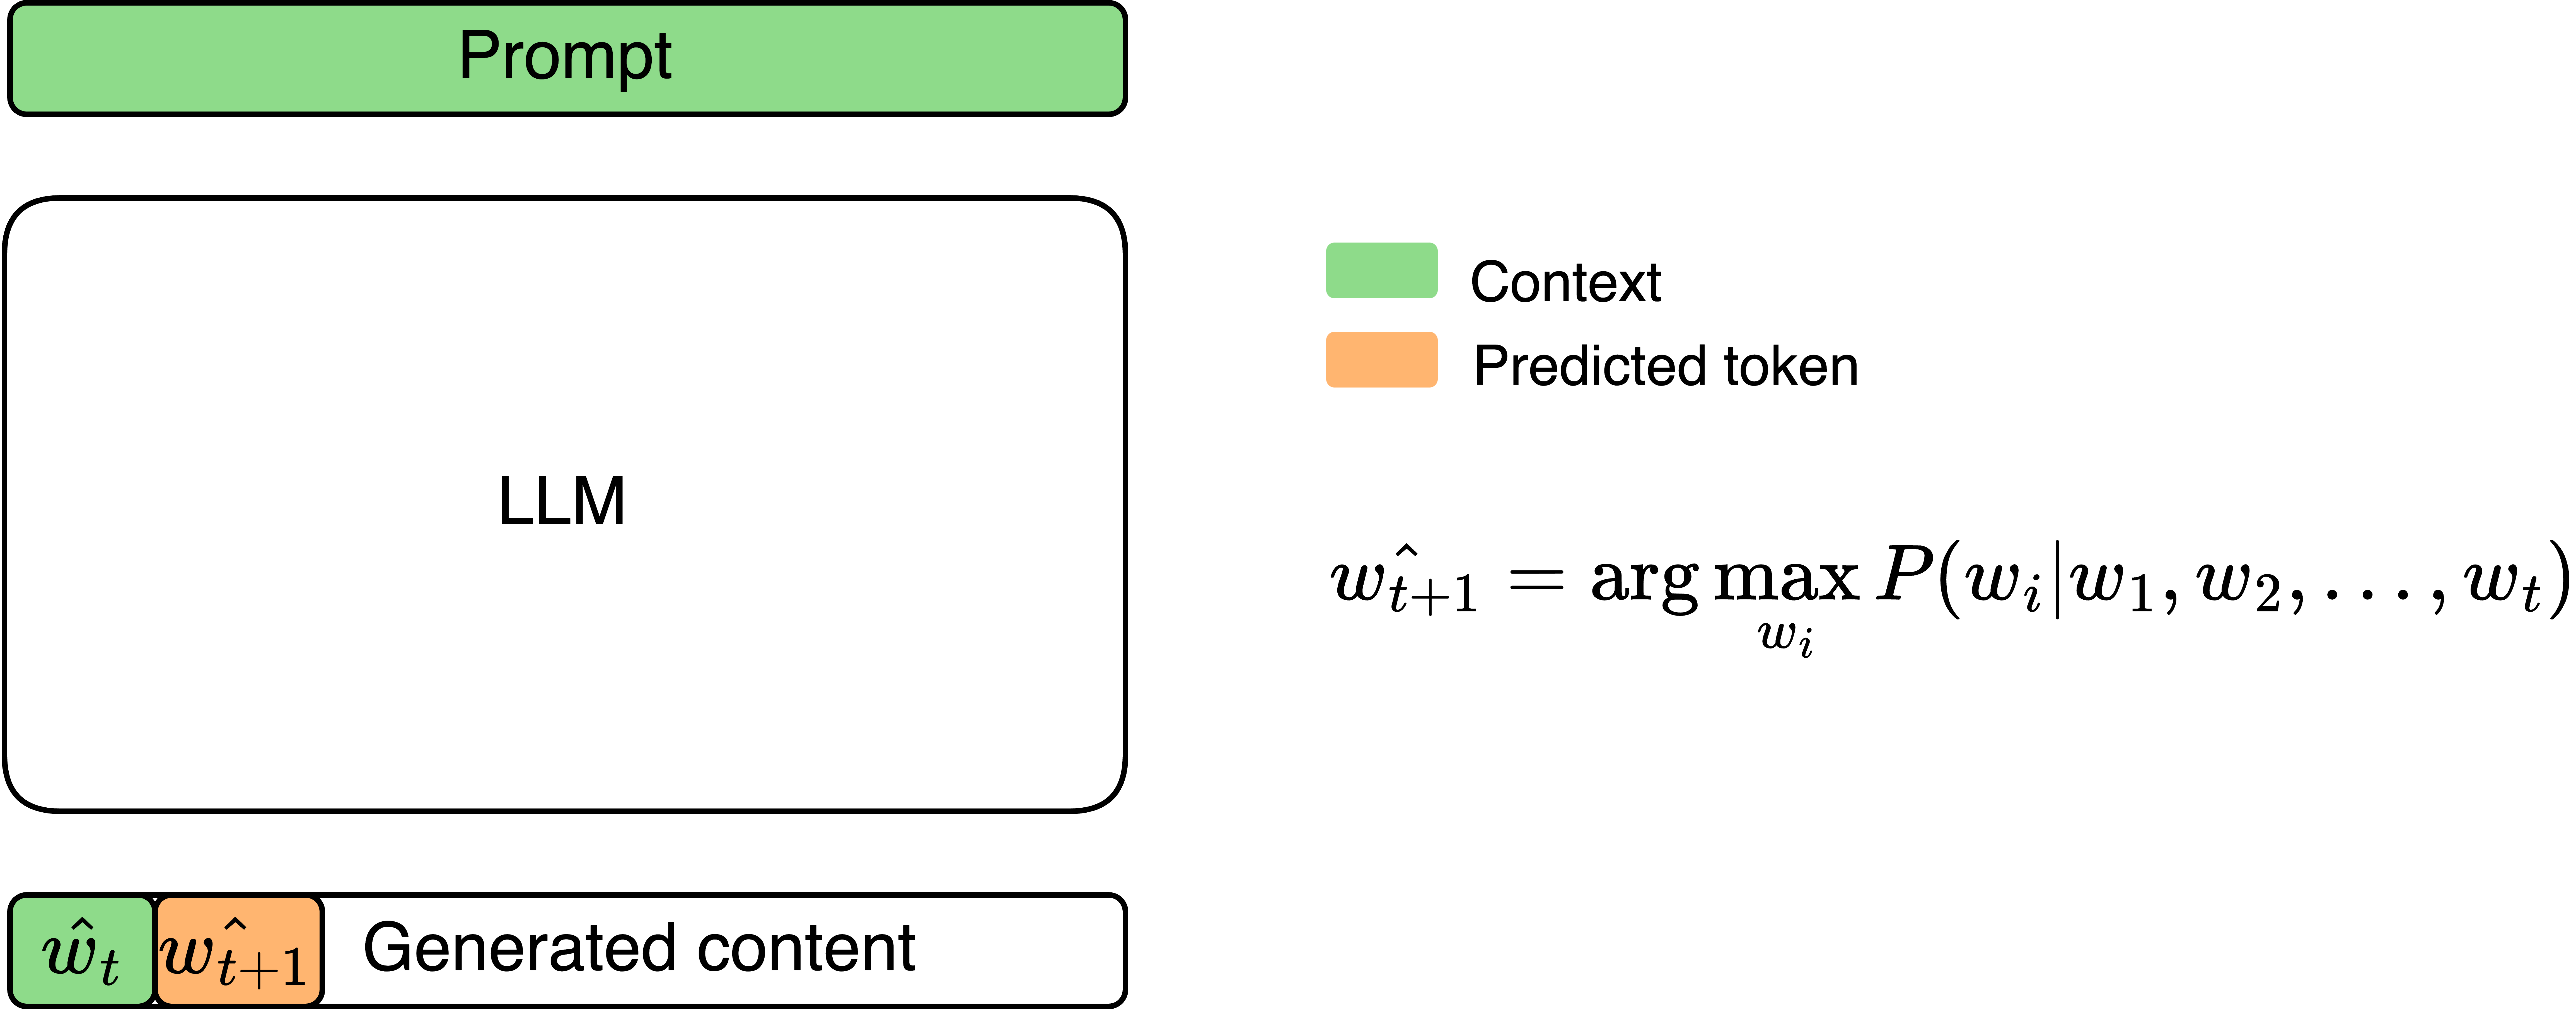
\includegraphics[width=0.9\textwidth]{llm_autoregressive_2.png}
    \end{figure}
    \begin{itemize}
        \item \textbf{Top p}: adjust the range of tokens to consider regarding their probability.
        \item \textbf{Top k}: choose among the $k$ more likely tokens. Default is 1 (most likely token).
        \item \textbf{Temperature:} control "creativity" by adding random noise to select less likely tokens.
    \end{itemize}
\end{frame}

% Now we know how information flows and is processed inside an LLM. We know better how it is inside.
% Ready to fine-tune that thing, but which guidelines should we follow

\begin{frame}{How Large are Large Language Models?}
    \begin{columns}
        \begin{column}{0.6\linewidth}
            \vspace{-0.1cm}
            \begin{table}[]
                \begin{tabular}{@{}llll@{}}
                    \toprule
                    Model       & Parameters & Layers & Context Size  \\ \midrule
                    Gemini 1.5  & 200B?      & -      & 10M  \\
                    GPT-4 turbo & 1.8T       & 120    & 128k            \\
                    Claude 2.1  & 12B        & -      & 200k            \\ \bottomrule
                \end{tabular}
                \caption{\centering Some \textsl{closed-source} model specifications}
            \end{table}
            \vspace{-0.4cm}
            \begin{table}[]
                \begin{tabular}{@{}llll@{}}
                \toprule
                Model        & Parameters & Layers & Context Size \\ \midrule
                Llama 3.3    & 70B        & 80     & 128k           \\
                Phi 4        & 14B        & 40     & 16k            \\
                Qwen 2.5     & 0.5B-72B   & 24-80  & 32k - 128k     \\
                Mistral-v0.3 & 7B         & 32     & 32k            \\ \bottomrule
                \end{tabular}
                \caption{\centering Some \textsl{open-weights} model specifications}
            \end{table}
        \end{column}
        \begin{column}{0.4\linewidth}
            \vspace*{-0.5cm}
            \begin{center}
            \textcolor{blue}{\sl Side remark: most LLMs called "open-source" are actually open-weights!}
            \end{center}
            \vspace{0.5cm}
            \begin{itemize}
                \item <2-> Most models involve several gigabytes in RAM GPU to perform inference
                \item <2-> Updating each parameter value during fine-tuning would be too costly
            \end{itemize}
            \vspace{0.3cm}
            \visible<2->{$\longrightarrow$ fine-tuning should be \textbf{efficient}}
        \end{column}
    \end{columns}
    
    
\end{frame}

\begin{frame}{Fine-Tuning is an \textsl{Affinage}: the Cheese Analogy}
    \visible<2>{
        \begin{figure}
            \centering
            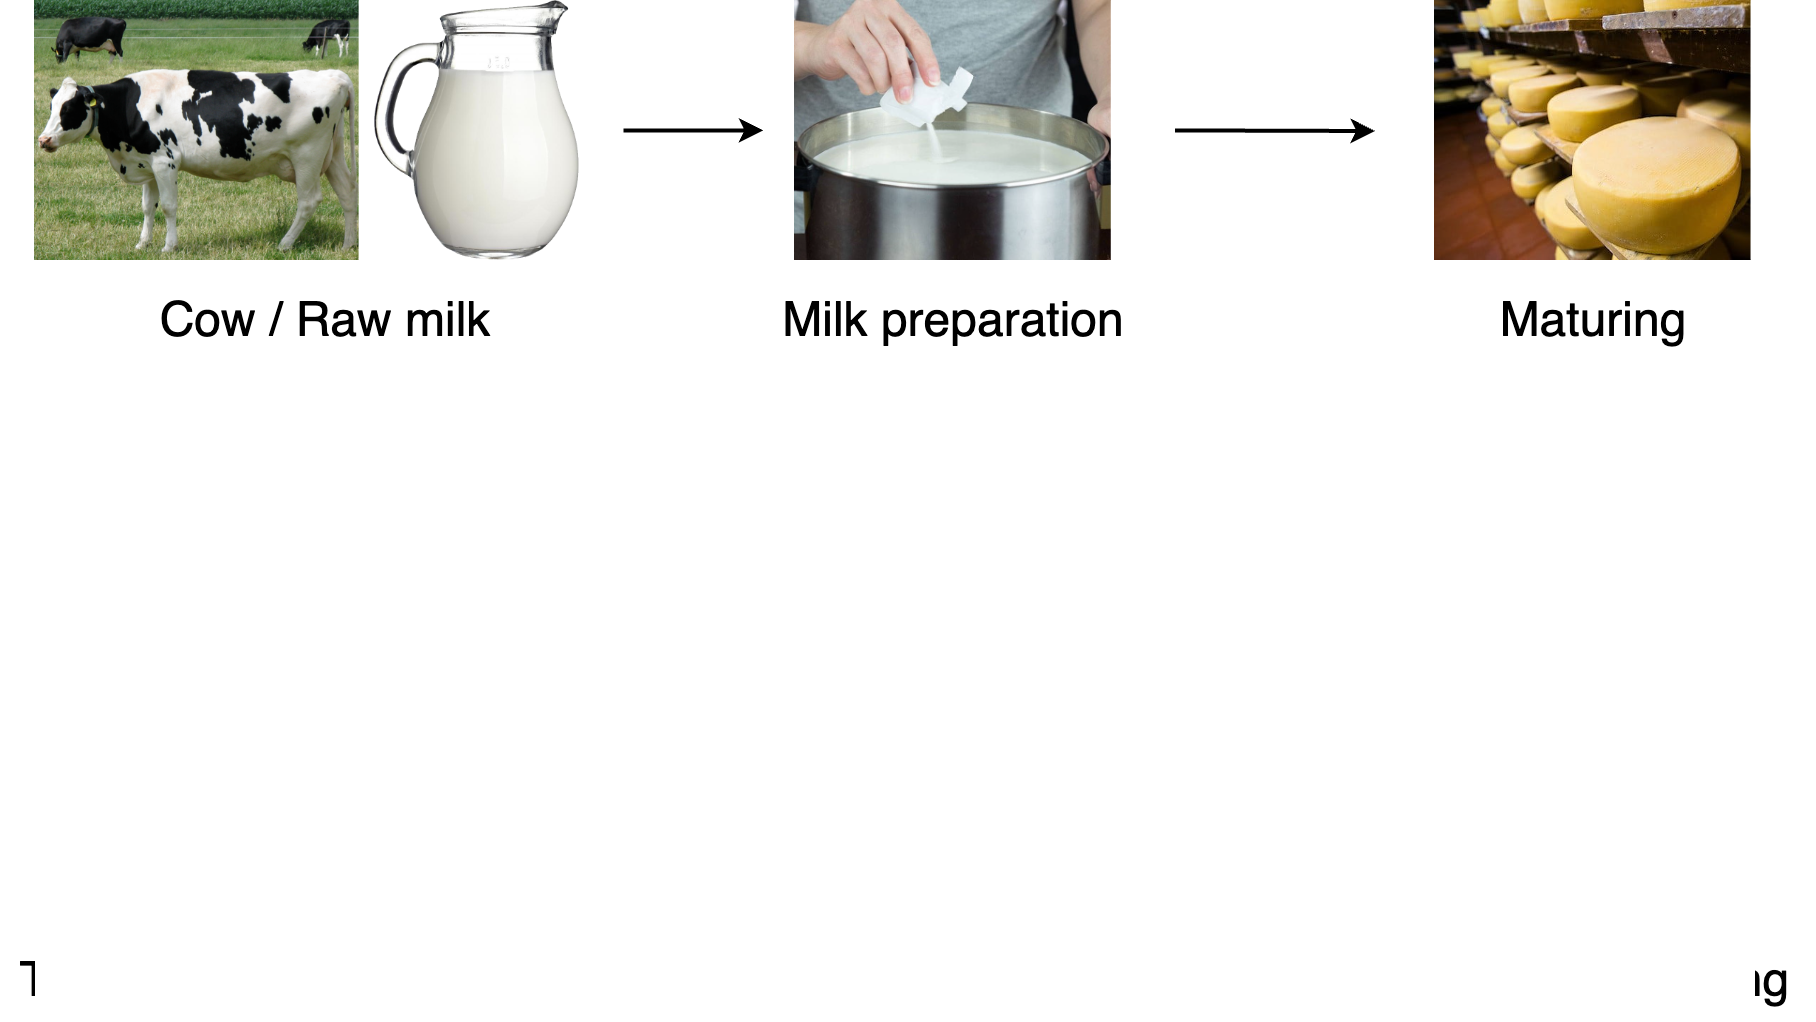
\includegraphics[width=0.8\textwidth]{pretrain_finetune_1.png}
        \end{figure}
    }
\end{frame}

\begin{frame}{Fine-Tuning is an \textsl{Affinage}: the Cheese Analogy}
    \begin{figure}
        \centering
        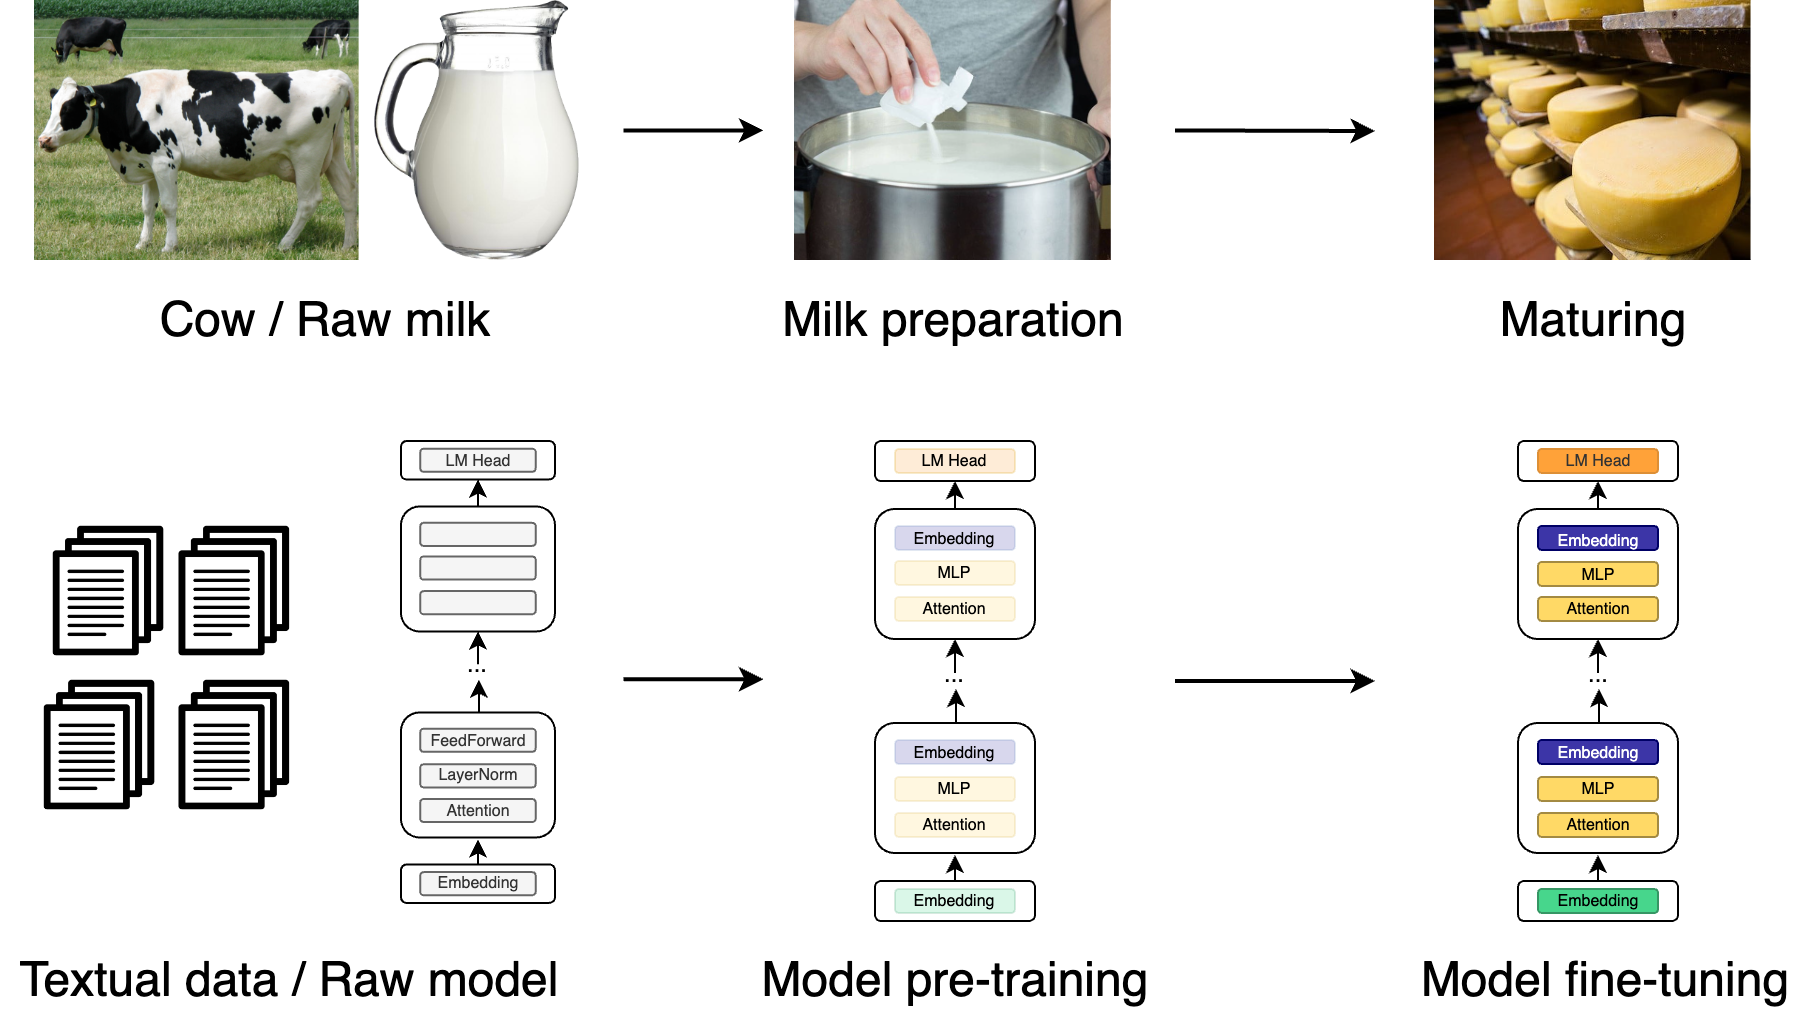
\includegraphics[width=0.8\textwidth]{pretrain_finetune_2.png}
    \end{figure}
\end{frame}

\begin{frame}{Fine-Tuning is an \textsl{Affinage}: the Cheese Analogy}
    \begin{figure}
        \centering
        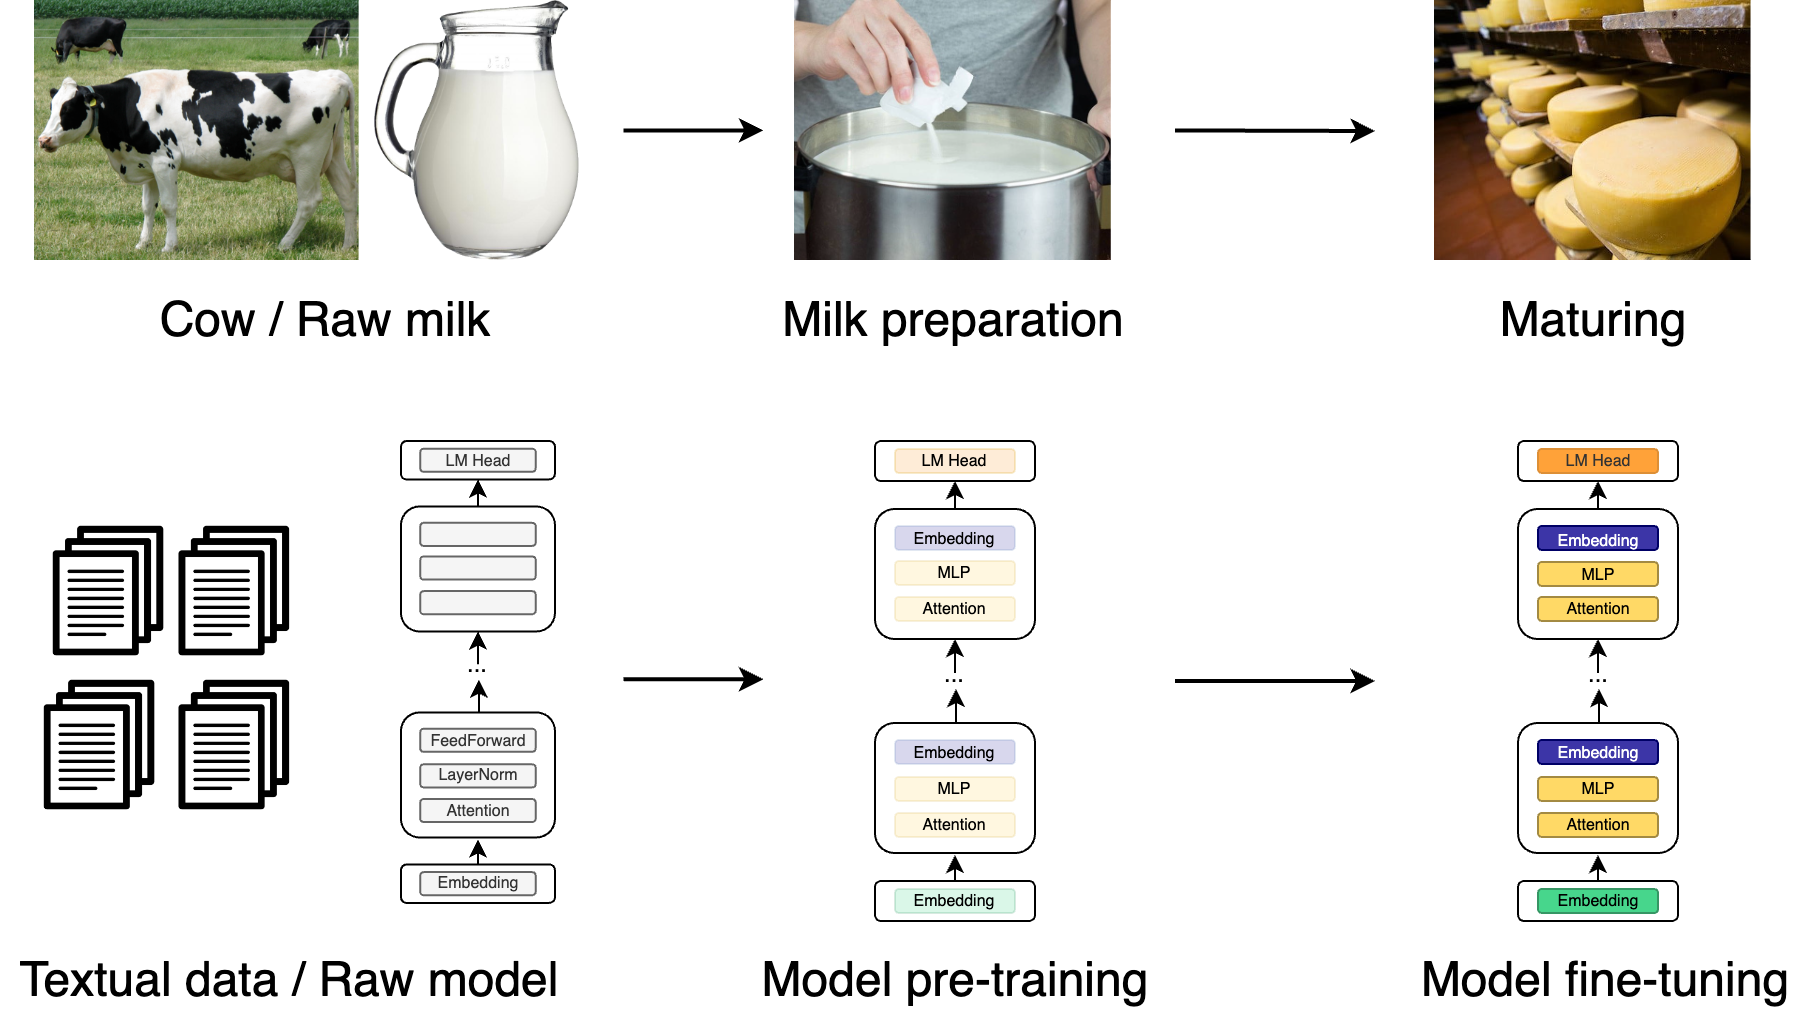
\includegraphics[width=0.4\textwidth]{pretrain_finetune_2.png}
    \end{figure}
    Fine-tuning, as cheese maturing phase, modifies \textbf{in place} its given instance.
    \begin{itemize}
        \item Ensure fine-tuning is performed in the right conditions
        \item Check pre-trained baseline reliability
        \item Test several (adapted) pre-trained baselines for one fine-tuning experiment
    \end{itemize}
    \visible<2->{$\longrightarrow$ fine-tuning should be \textbf{stable} and \textbf{consistent} with pre-trained baseline}
\end{frame}


\begin{frame}{Efficient Fine-Tuning With Adapters~\cite{houlsby2019parameterefficienttransferlearningnlp}}
    \begin{columns}
        \begin{column}{0.5\linewidth}
            \vspace{-0.2cm}
            \begin{figure}
                \centering
                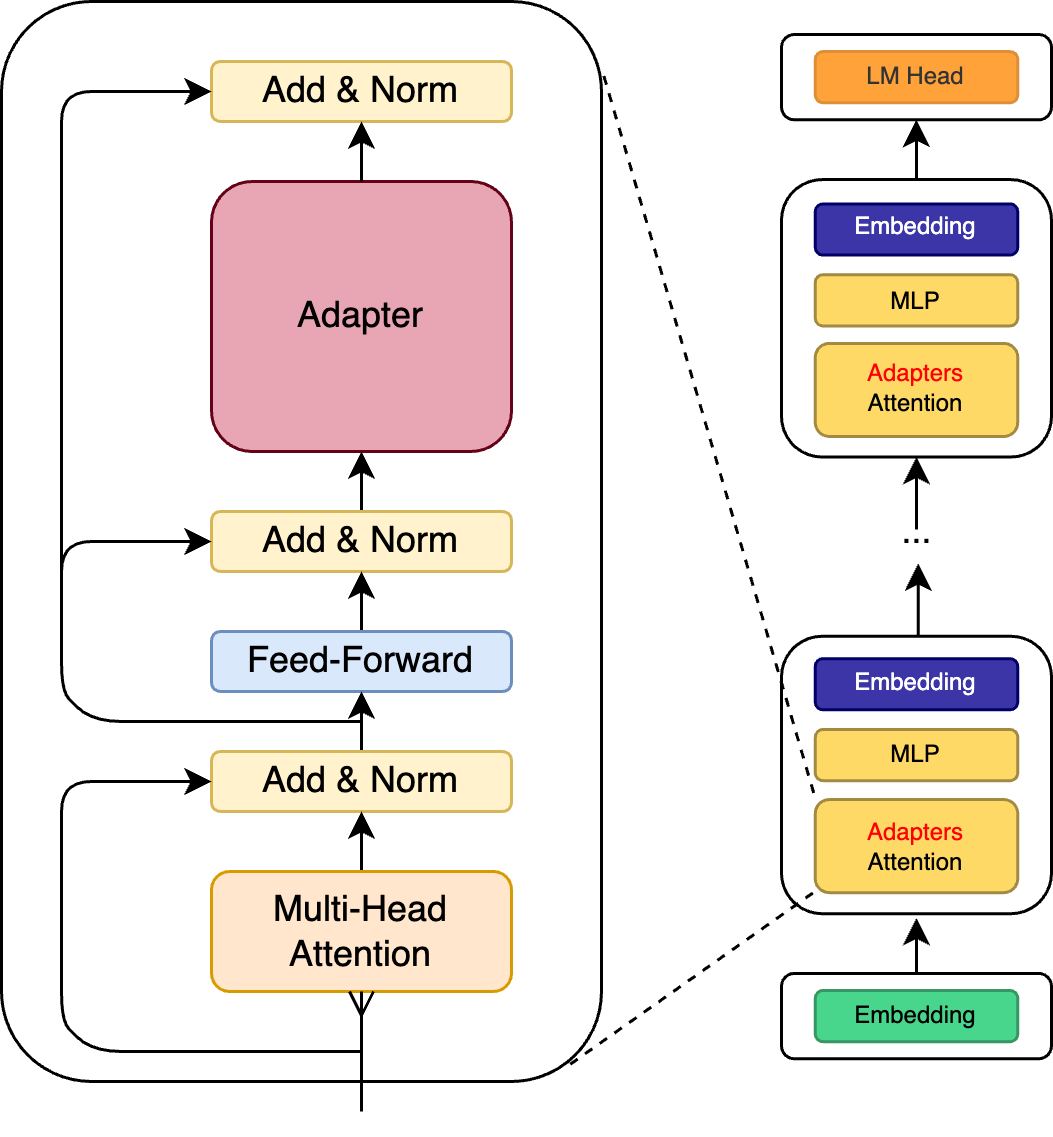
\includegraphics[width=0.8\textwidth]{llama-adapter-simple.png}
                \caption{\centering An attention block with adapters}
            \end{figure}
        \end{column}
        \begin{column}{0.5\linewidth}
            \vspace{-0.2cm}
            \begin{center}
            \textbf{Adapters layers are inserted to enable parameter-efficient fine-tuning\footnote{\scriptsize\url{https://huggingface.co/PEFT}}}
            \end{center}
            % \vspace{0.1cm}
            Common usage:
            \begin{itemize}
                \item Freeze all pre-trained model layers
                \item Insert trainable MLP layers into attention blocks (query, value) and/or model head
            \end{itemize}
            \vspace{0.1cm}
            \visible<2->{Advantages:
            \begin{itemize}
                \item Fewer param. updates than full fine-tuning
                \item Helps reduce catastrophic forgetting~\cite{DBLP:journals/corr/abs-2005-00247}
                \item Easy to share fine-tuned models\footnote{\scriptsize\url{https://adapterhub.ml/}}
            \end{itemize}
            }
        \end{column}
    \end{columns}
\end{frame}

\begin{frame}{Efficient Fine-Tuning With LoRA Adapters~\cite{hu2021loralowrankadaptationlarge}}
    \begin{columns}
        \begin{column}{0.5\linewidth}
            \vspace{-0.2cm}
            \begin{figure}
                \centering
                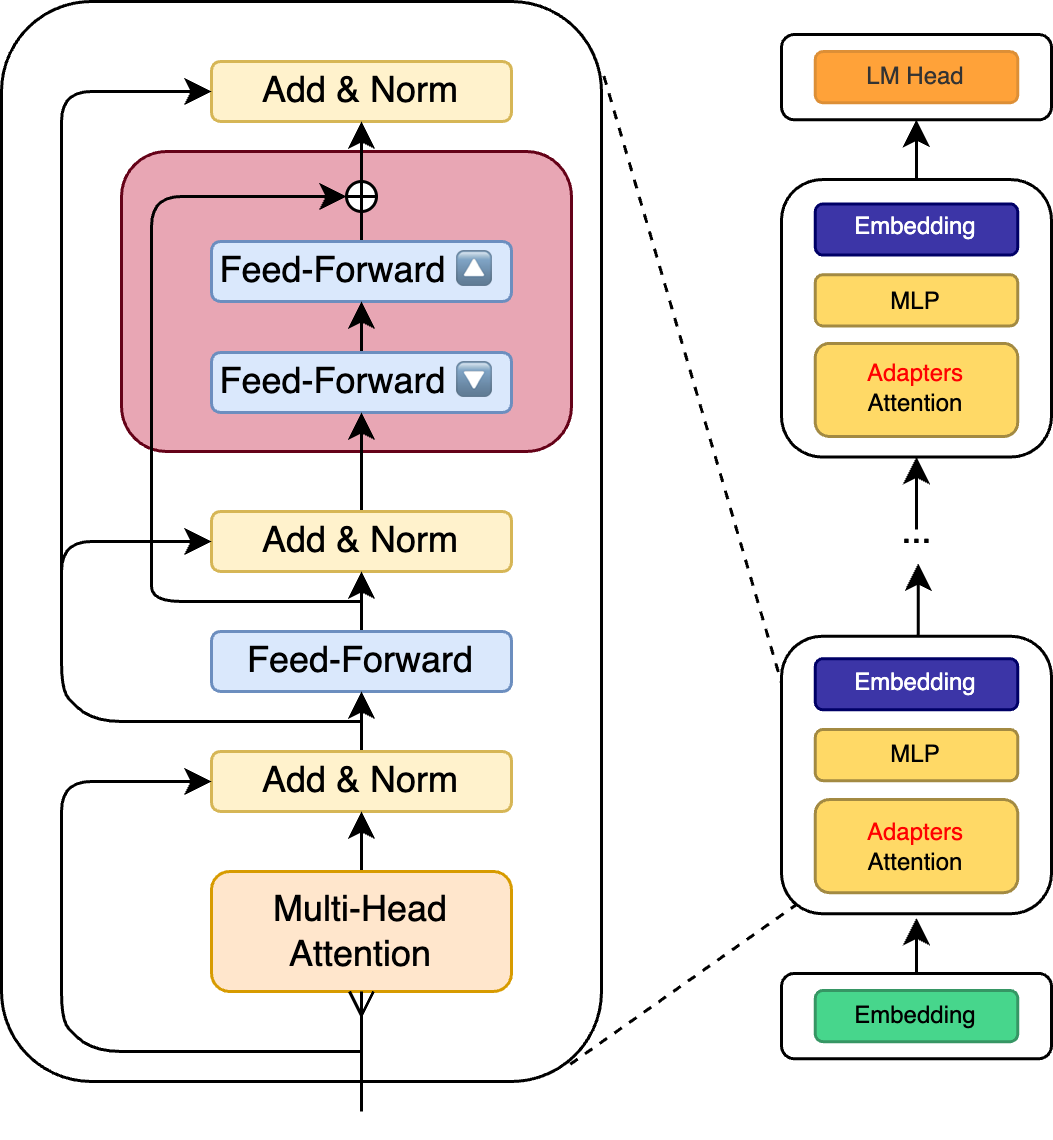
\includegraphics[width=0.8\textwidth]{llama-adapter.png}
                \caption{\centering An attention block with LoRA adapters}
            \end{figure}
        \end{column}
        \begin{column}{0.5\linewidth}
            \vspace{-0.5cm}
            \begin{center}
            \textbf{LoRA: Low-Rank Adaptation\\A specific adapter block structure}
            \end{center}
            \vspace{0.1cm}
            \begin{itemize}
                \item Information from the model can be represented (almost) equally well in a lower dimensional space
                \item The rank $r$ of the lower dim. space should be determined by hyperparameter tuning
                \item Quantized versions: QLoRA~\cite{dettmers2023qloraefficientfinetuningquantized}
            \end{itemize}
        \end{column}
    \end{columns}    
\end{frame}

\begin{frame}[plain]
    \begin{center}
        \vspace{0.5cm}
        {\color{roose}\Huge Thanks for your attention!}
        
        \vspace{0.3cm}
        
        \begin{figure}[h]
            \centering
            
\includegraphics[width=0.4\textwidth]{qr_code.png}
            \caption{\centering Practical session: \url{https://github.com/B-Gendron/tutorial-deeploria/lab/}}
        \end{figure}
    \end{center}
\end{frame}

\begin{frame}[t,allowframebreaks,noframenumbering]
    \frametitle{References}
    \printbibliography
\end{frame}

% - Petit point d'étape, prise de recul. Déjà, "Large" comment ("How large and Large Language Models?")
%     - Donner des valeurs chiffrées pour donner des repères aux gens, ainsi que des temps d'exécution indicatifs et les requirements CPU/GPU pour faire des choses classiques. Ne présenter que les LLMs open-source et en profiter pour dire que les modèles type GPT, Claude etc. sont closed-source donc on ne sait pas
%     - Autre point de détail au passage: open-source / open-weight ("Open-source or open-weights?")
% - Paradigme pré-entraînement / affinage, parallèle fromage
%     - On arrive à la problématique du fine-tuning
% - Comment faire un fine-tuning efficace?
%     - On a vu le temps que ça prenait de mettre à jour tous les paramètres donc on n'a pas envie de faire ça
%     - Ne mettre à jour que certains paramètres : comment les choisir ? 
%     - Adapters, Low-Rank Adaptation
%         - Explication du concept des adapters
%         - Description du principe de LoRA
%         - Présentation d'adapters hub (bien préciser que les adapters sont modèle dépendants)


\end{document}